\documentclass[11pt,spanish]{article}

%----------------------------------------------------------------------------------------
% Codificación, y usar una fuente similar a la Palatino (y no Latin Modern Roman)
\usepackage[utf8]{inputenc} % Acentos, etc.
\usepackage[spanish]{babel} % Castellano
\usepackage{tgpagella}      % Fuente similar a Palatino
\usepackage[T1]{fontenc}

%----------------------------------------------------------------------------------------
% TODO
\usepackage{color}
\newcommand{\TODO}[1]{\textcolor{red}{\textbf{\MakeUppercase{#1}}}}

%----------------------------------------------------------------------------------------
% Enumerate with dash instead of period
\usepackage{enumitem}

\makeatletter
\def\twodigits#1{\expandafter\@twodigits\csname c@#1\endcsname}
\def\@twodigits#1{%
  \ifnum#1<10 0\fi
  \number#1}
\makeatother
\AddEnumerateCounter{\twodigits}{\@twodigits}{100}

%----------------------------------------------------------------------------------------
% Indentar primera línea párrafos
\usepackage{indentfirst}


%----------------------------------------------------------------------------------------
% MODIFICAR EL ESTILO DE LAS SECCIONES 
\usepackage{titlesec}
\titleformat{\section}{\bfseries\Large}{\thesection}{0.8em}{}
\titleformat{\subsection}{\bfseries\large}{\thesubsection}{0.8em}{}
\titleformat{\subsubsection}{\bfseries\large}{\thesubsubsection}{0.8em}{}
%\newcommand{\sectionbreak}{\clearpage} % Empezar secciones en nueva página


%----------------------------------------------------------------------------------------
% Footnotes without line
\makeatletter
\newcommand\footnoteref[1]{\protected@xdef\@thefnmark{\ref{#1}}\@footnotemark}
\makeatother

%----------------------------------------------------------------------------------------
% Imagenes: Que se pongan donde yo quiero
\usepackage{graphicx}
%\usepackage{float}
\usepackage[linecolor=colComment,linewidth=0.65pt]{mdframed}

\DeclareGraphicsExtensions{.svg,.eps,.ps,.pdf,.png,.jpg,.jpeg}
\addto{\captionsspanish}{\renewcommand{\listfigurename}{\bfseries\Large Figuras}}

%----------------------------------------------------------------------------------------
% Poder insertar .pdf en .tex
\usepackage{pdfpages}

%----------------------------------------------------------------------------------------
% Cronograma: Diagrama de Gantt
\usepackage{gantt}
% Cronograma girado 90º
\usepackage{rotating}
\usepackage{fixltx2e} % poder poner 1ª en modo texto (no matemático)


%----------------------------------------------------------------------------------------
% COLORES
\usepackage{xcolor}

% Paleta 1
\definecolor{fucsia_P1}{RGB}{105,45,172}
\definecolor{naranja_P1}{RGB}{255,153,0}
\definecolor{verde_P1}{RGB}{87,190,133}
\definecolor{rojo_P1}{RGB}{216,117,117}
\definecolor{azul_P1}{RGB}{51, 102, 153}
\definecolor{gris_P1}{RGB}{143,145,148}
%----------------------------------------------------------------------------------------
% Comenzar con numeracion romana (I,II,III,IV,...)
\renewcommand{\thepage}{\roman{page}}

%----------------------------------------------------------------------------------------
% Definir el titulo

\newcommand{\nombreDelProyecto}{$\mu Search$}

% Comando para multiples saltos de linea
\newcommand{\singlelinebreak}{\\[\baselineskip]}
\newcommand{\multiplelinebreak}[1]{\\[#1\baselineskip]}
\newlength{\drop}

\newcommand*{\titulo}{\begingroup
\thispagestyle{empty}
\drop = 0.13\textheight
\centering
\vfill
\vspace*{\drop}

\includegraphics[scale=0.25]{img/bitparty_big}\singlelinebreak
{\Huge\bf BITPARTY}\multiplelinebreak{2}
{\huge Proyecto \nombreDelProyecto}\multiplelinebreak{2}
{\Large Versión  1.0}\multiplelinebreak{1}
{\Large 03/2014}
\vfill
\vspace*{\drop}
\endgroup}


%----------------------------------------------------------------------------------------
% METADATOS DEL PDF Y PDF CLICKEABLE
\usepackage{hyperref}
\usepackage{hyperxmp}

\hypersetup{
	pdfauthor={Alberto Berbel Aznar, 
				Javier Briz Alastrué, 
				Héctor Francia Molinero, 
				Daniel García Páez,
				Alejandro Gracia Mateo,
				Simón Ortego Parra},
	pdftitle={E20 - Propuesta del proyecto},
	pdfsubject={Proyecto Software. Grado Ing. Informática. EINA. Unizar},
	pdfkeywords={},
	pdfcopyright={Copyright (C) 2014 by Alberto Berbel Aznar, 
				Javier Briz Alastrué, 
				Héctor Francia Molinero, 
				Daniel García Páez,
				Alejandro Gracia Mateo,
				Simón Ortego Parra. All rights reserved.},
	pdfproducer={PDFLatex},
	pdfcreator={ps2pdf},
	colorlinks=false
}

\usepackage[capitalise]{cleveref} % load after hyperref package
\crefdefaultlabelformat{\textbf{#2#1#3}} % boldface only the number

\crefname{figure}{figura}{figuras}
\Crefname{figure}{Figura}{Figuras}

\crefname{listing}{algoritmo}{algoritmos}
\Crefname{listing}{Algoritmo}{Algoritmos}

\crefname{section}{sección}{secciones}
\Crefname{section}{Sección}{Secciones}

%----------------------------------------------------------------------------------------
% FANCY HEADER
\usepackage[head=34pt]{geometry}

\usepackage{fancyhdr}
\pagestyle{fancy}
\fancyhf{} % borrar todos los ajustes

% Configurar la cabecera: fancyhead, fancyfoot para el pie.
\fancyhead[L]{\nouppercase\leftmark}
\fancyhead[R]{\nouppercase\rightmark\hspace{0.5em}}
\fancyfoot[C]{-- \thepage\ --}

% Cabecera parte derecha: número y título de sección, subsección, etc.
\renewcommand{\sectionmark}[1]{\markright{\small{{\bf \thesection} - #1}}}
\renewcommand{\subsectionmark}[1]{\markright{\small{{\bf \thesubsection} - #1}}}
\renewcommand{\subsubsectionmark}[1]{\markright{\small{{\bf \thesubsubsection} - #1}}}

% Cabecera parte izquierda: Nombre de la empresa (logo) y nombre del proyecto
\lhead{\raisebox{-0.5\height}{\rule[-.5ex]{0pt}{2ex}
\includegraphics[scale=0.125]{img/bitparty_small}}\hspace{1em}{\large\nombreDelProyecto}}

\renewcommand{\headrulewidth}{0.6pt} % Tam. separador cabecera
\renewcommand{\footrulewidth}{0pt}   % Tam. separador pie
\renewcommand{\headwidth}{6in}       % Anchura cabecera (incluido separador)

%----------------------------------------------------------------------------------------
%----------------------------------------------------------------------------------------
% INICIO DEL DOCUMENTO
%----------------------------------------------------------------------------------------


%----------------------------------------------------------------------------------------
% PORTADA: TÍTULO
%----------------------------------------------------------------------------------------
\begin{document}
\titulo
\clearpage


%----------------------------------------------------------------------------------------
% ABSTRACT: RESUMEN EJECUTIVO
%----------------------------------------------------------------------------------------
\thispagestyle{empty}
\null\vspace{\fill}
\begin{abstract}
\paragraph{} Se presenta en este documento la propuesta de proyecto  para el desarrollo de una aplicación web para la venta de microcontroladores a través de un catálogo electrónico, tal y como nos pedía el cliente.
\paragraph{} La aplicación web permite al cliente la búsqueda de microcontroladores en un catálogo electrónico existente, mostrando como resultado un listado sin paginación. 
\paragraph{} El cliente puede añadir desde dicho listado a su carrito de compra los microcontroladores que desee y modificar posteriormente las unidades finales en el carrito de compra, para así poder pedir finalmente la generación de un presupuesto en formato PDF. Cabe recalcar que cada vez que un cliente desee generar un pedido debe introducir sus datos personales y de empresa, es decir, no hay persistencia de los datos.
\paragraph{} Se proporciona además una interfaz web exclusiva para los administradores, a la que solo se accederá desde la empresa cliente de manera local, que tendrán permiso para añadir nuevos microcontroladores al catálogo y modificar y/o eliminar los ya existentes.
\paragraph{} La aplicación entregada a la empresa cliente incluye el servidor web y de base de datos en completo funcionamiento, siendo esto una gran aliciente para la adquisición del producto, pues evita un gasto importante a la empresa cliente. 
\paragraph{} El diseño arquitectural de la aplicación está basado en el patrón Modelo-Vista-Controlador, en concreto, la variante Modelo-Vista-Presentador, separando así de manera notable la vista de la aplicación de los datos de la aplicación, escondiendo así al usuario todos los detalles internos para mayor seguridad de la aplicación.
\paragraph{} En cuanto a detalles tecnológicos de la implementación, concretar que la interfaz web estará implementada con HTML5, CSS3 integrado con el control implementado en PHP5 utilizando el framework CodeIgniter2.1.4 y que se comunica con una base de datos en MySQL5.5. Se asegura además que la aplicación funcionará correctamente en varios de los navegadores web más actuales (Chrome, Mozilla, Opera…).
\paragraph{} Ya presentados los detalles de funcionamiento e implementación de la aplicación, se presentan en el punto final del documento:
\begin{itemize}
\item La división de tareas del proyecto junto a un datagrama, proveyendo así al cliente de una idea bastante exacta de los cumplimientos de plazos previstos.
\item Una oferta económica del desarrollo total de la aplicación.
\end{itemize}

\end{abstract}

\vspace{\fill}
\newpage


%----------------------------------------------------------------------------------------
% ÍNDICE
%----------------------------------------------------------------------------------------	
\tableofcontents
\clearpage


% Continuar con numeracion romana (1,2,3...) 
\renewcommand{\thepage}{\arabic{page}}
%----------------------------------------------------------------------------------------
% 1. IDENTIFICACIÓN DEL PROYECTO
%----------------------------------------------------------------------------------------
\section{Identificación del proyecto}
\noindent{
	Identificamos el proyecto y su funcionalidad con el siguiente título:
	\begin{flushleft}
		\textbf{\large \\ Página web para la venta de microcontroladores a través de un \newline catálogo electrónico}
	\end{flushleft}

}
	
\noindent{	
	\\
	Además del título, se ofrece la posibilidad de identificar el proyecto a través del siguiente codigo:
	\begin{center}
		\textbf{\textit{\large \\ ps-14-e20-usearch}}
	\end{center}
	Donde:
		\begin{itemize}
		\renewcommand{\labelitemi}{$\bullet$}
			\item ''ps'' hace referencia a ''Proyecto Software''
			\item ''14'' hace referencia al año 2014
			\item ''e20'' hace a referencia al equipo del proyecto, ''Equipo 20''
			\item ''usearch'' hace referencia al nombre del proyecto
		\end{itemize}
}

%----------------------------------------------------------------------------------------
% 2. DATOS DEL LICITADOR
% 2.1 DENOMINACIÓN DE LA EMPRESA
% 2.2 HISTORIAL DEL EQUIPO
%----------------------------------------------------------------------------------------
\section{Datos del licitador}
\input{tex/02_0_datos_del_licitador}

\subsection{Denominación de la empresa}
La empresa emisora de la presente propuesta se denomina:
\begin{center}
        \textbf{\textit{\large \\ BitParty}}
\end{center}
Esta emprese se dedica al desarrollo de software, especialmente de aplicaciones web orientadas a pequeñas y medianas empresas para la gestión de su catalogo y tienda online.
\newpage


\subsection{Historial del equipo}

\paragraph{} El equipo cuenta con experiencia en:
\begin{itemize}

\item El mantenimiento de administración de sistemas.
\item El desarrollo y mantenimiento de sistemas web utilizando diferentes lenguajes como HTML, PHP, CSS, JavaScript.
\item La administración de gestores de contenidos como Drupal, Wordpress... 
\item El desarrollo y mantenimiento de bases de datos.
\item Montar web con funcionalidades similares con gestión de contenido como películas o series.

\end{itemize}

\begin{itemize}

\item Amplia experiencia en el ámbito de la web.
\item Conocimiento de entornos cliente-servidor.
\item Creación de interfaces web.

\end{itemize}


%----------------------------------------------------------------------------------------
% 3. OBJETO DE LA PROPUESTA
%----------------------------------------------------------------------------------------
\section{Objeto de la propuesta}
La presente aplicación trata de dar solución al problema planteado por la empresa cliente.
El cliente nos ha transmitido la necesidad de diseñar un catálogo electrónico de los microconroladores que distribuye, que permita la gestión de los productos disponibles, y que permita a los clientes realizar búsquedas y efectuar pedidos.



%----------------------------------------------------------------------------------------
% 4. REQUISITOS DEL SISTEMA
%----------------------------------------------------------------------------------------
\section{Requisitos del sistema}
\documentclass[10pt,a4paper]{article}
\usepackage[T1]{fontenc}
\usepackage[utf8]{inputenc}
\usepackage[spanish]{babel}
\begin{document}

\section{Requisitos}
\begin{enumerate}

\item Un microcontrolador (elemento) estará compuesto de los siguientes campos: 
	\begin{enumerate}
		\item Referencia (será única para cada elemento).
        \item Arquitectura
        \item Frecuencia
        \item Flash
        \item RAM
        \item Precio
	\end{enumerate}
	
\item Insertar un elemento en el carro de compra.
   
\item Eliminar un elemento del carro de compra.
	
\item Modificar un elemento del carro de compra. Por modificar se entiende alterar el número de unidades de los elementos.

\item Se podrá acceder a los elementos del catálogo mediante un listado en el que aparezcan todos sus elementos.

\item Se podrá actualizar varios elementos del carro de manera simultánea. Por actualizar se entiende a recalcular los precios de cada artículo en el caso de que éstos hayan sido modificados.

\item Se permitirá realizar búsquedas de productos en función de un único campo de búsqueda y en base a una de las características de los elementos. 
	
\item Los resultados de la búsqueda se presentarán como un listado (sin paginación) que mostrará, de cada elemento, todos sus campos en columnas.

\item Se permitirá realizar pedidos en los que se incluirán los datos del cliente cada vez. Es decir, no existirá persistencia de los datos del cliente tras realizar pedidos.

\item Los pedidos contendrán la suficiente información para identificar a los clientes. Además, no permitirán la reserva de los productos solicitados, únicamente generarán un presupuesto con el coste de los productos elegidos.

\item Los datos solicitados del cliente para los pedidos serán los siguientes:

	\begin{enumerate}
		\item Nombre 
		\item Apellidos
	    \item Dirección
	    \item Ciudad
	    \item Provincia
	    \item País
	    \item Código postal
	    \item Teléfono
	    \item Correo electrónico
	    \item CIF y Empresa aparecerán como campos opcionales que servirán de distinción entre particulares y entidades.
	\end{enumerate}
	

\item Se contará con una vista diferente para la administración del catálogo a la que no podrán acceder los clientes (se ejecutará solamente en local). 
En ésta vista se podrán realizar las acciones de:
	
	\begin{enumerate}
    	\item Insertar un elemento en el catálogo (a partir de las
           arquitecturas disponibles, no se permitirá añadir nuevas
           arquitecturas al catálogo).  
		\item Eliminar un elemento del catálogo.
        \item Modificar un elemento del catálogo. En éste caso, modificar un elemento del catálogo sería cambiar cualquiera de sus características.
    \end{enumerate}   

\end{enumerate}
\end{document}



%----------------------------------------------------------------------------------------
% 5. DESCRIPCIÓN TÉCNICA DE LA SOLUCIÓN PROPUESTA
% 5.1. ESQUEMA DE LA ARQUITECTURA
% 5.2. TECNOLOGÍAS 
%----------------------------------------------------------------------------------------
\section{Descripción técnica de la solución}
Se propone una solución basada en tecnologías web, capaces de resolver tanto los requisitos de interacción de la aplicación con el usuario como los problemas relacionados con tratamiento y persistencia interna de la información.
Concretamente, se utilizará una interfaz web compatible con las últimas versiones de los navegadores más utilizados (más adelante se detallará esto), y se utilizará el framework CodeIgniter, en lenguaje PHP, como base del proyecto. Para el almacenamiento de la información se utilizará una base de datos MySQL.
Para evitar problemas de latencias con la base de datos, y dado el reducido tamaño del sistema, se optará por alojar la base de datos y todo el resto del sistema (servidor web e intérprete PHP) en un mismo servidor.

Las tecnologías, lenguajes y aplicaciones propuestas para el desarrollo del proyecto son:

\begin{itemize}
\item HTML 5
\item CSS 3
\item PHP 5
\item CodeIgniter 2.1.4
\item MySQL 5.5
\end{itemize}

Se asegurará que la web renderice de forma correcta en los siguientes navegadores:

\begin{itemize}
\item Google Chrome >=30
\item Internet Explorer >=10
\item Mozilla Firefox >=27
\item Opera >=12
\end{itemize}

La documentación y manuales de usuario se entregarán al cliente en PDF.



\subsection{Esquema de la arquitectura}
\paragraph{}El patrón que vamos a utilizar para el diseño arquitectural de nuestro 
catálogo va a ser el de Modelo-Vista-Controlador, en contreto, la variante Modelo-Vista-Presentador.

\vspace{.2cm}
\begin{figure}[h!]
 \centering
 \includegraphics[scale=.6]{../img/diagrama_desplieque}
 \caption{Diagrama de despliegue del sistema}
\end{figure}
\vspace{.2cm}


\paragraph{Interfaz web}Es nuestro componente vista, lo que utilizan los usuarios para 
interactuar con la aplicación y visualizar los resultados que producen dichas
interacciones. Las acciones del usuario que impliquen el acceso o la modificación
de los datos del modelo son delegadas al componente Controlador.

\paragraph{Controlador}Es nuestro componente Presentador, tiene toda la lógica de la vista 
y es responsable de sincronizar el modelo y la vista. Cuando la vista notifica el 
presentador que el usuario ha hecho algo (por ejemplo, hacer clic en un botón), 
el presentador a continuación, actualiza el modelo y sincroniza los cambios 
entre el modelo y la vista.

\paragraph{Es Base de datos}Es nuestro componente modelo, se encarga de encapsular 
los datos y ofrecer operaciones para su acceso y procesamiento. Solo el componente
Controlador interactúa con este componente.

\subsection{Tecnologías}
\input{tex/05_2_tecnologias}


%----------------------------------------------------------------------------------------
% 6. METODOLOGÍA DE GESTIÓN Y PLANIFICACIÓN
% 6.1. FASES Y ACTIVIDADES DEL PROYECTO
% 6.2. RECURSOS HUMANOS
% 6.3. CRONOGRAMA
% 6.4. PRESUPUESTO
%----------------------------------------------------------------------------------------
\section{Metodología de gestión y planificación del proyecto}
\input{tex/06_0_metodologia_de_gestion_y_planificacion}

\subsection{Fases y actividades del proyecto}
\paragraph{} El proyecto se divide en tres fases principales:
\begin{enumerate}
	\item Lanzamiento del proyecto.
	\item Primera iteración del proyecto.
	\item Segunda iteración del proyecto.
\end{enumerate}

\paragraph{} Se desarrollan a continuación las actividades o tareas que componen cada una de las fases:
\begin{enumerate}
	\item \textbf{Lanzamiento del proyecto.}
		\begin{itemize}
		\item Proceso de obtención de los requisitos funcionales y no funcionales de la aplicación.
		\item Diseño de un prototipo sin funcionalidad de la interfaz web de la aplicación.
		\item Diseño de la base de datos con la que trabajará la aplicación.
		\item Instalación  y puesta a punto del sistema sobre el que funcionará la aplicación.
		\item Planificación del datagrama de actividades para las dos iteraciones del proyecto y realización de un presupuesto.
		\end{itemize}
	\item \textbf{Primera iteración del proyecto.}
		\begin{itemize}
		\item Población de la base de datos.
		\item TAREA 1: Implementación básica de la interfaz web de la aplicación.
		\item TAREA 2: Implementación del control para insertar, modificar y eliminar elementos en el catálogo.
		\item TAREA 3: Implementación del control para mostrar listados de elementos del catálogo.
		\item TAREA 4: Implementación del control para el carrito de compra de la aplicación.
		\item TAREA 5: Implementación del control para generar, en texto plano, pedidos de compra.
		\item Documentación técnica de todo lo implementado (documentación de codigo y mantenimiento de una \textit{Wiki}.)
		\item Documentación del manual y guía de usuario de lo implementado hasta el momento.
		\item Preparación y realización de pruebas.
		\end{itemize}
	\item \textbf{Segunda iteración el proyecto.}
		\begin{itemize}
		\item Población de la base de datos.
		\item TAREA 6: Implementación del control para realizar búsquedas en el catálogo.
		\item TAREA 7: Implementación del control para generar pedidos de compra en formato PDF.
		\item TAREA 8: Mejora de la implementación inicial de la interfaz web de la aplicación
		\item Documentación técnica de todo lo implementado (documentación de codigo y mantenimiento de una \textit{Wiki}.)
		\item Documentación del manual y guía de usuario final.
		\item Preparación y realización de pruebas.
		\item Cierre y puesta a punto final del proyecto.
		\end{itemize}
\end{enumerate}
\paragraph{} Se puede observar una clara relación entre los requisitos del sistema definidos anteriormente y las tareas ''TAREA X'' aquí definidas. Pues es de esa forma como se ha abordado la planificación de tareas y actividades.
\paragraph{}Además, las tareas de documentación y pruebas son comunes a ambas iteraciones y se realizan paralelamente a la implementación con la intención de adelantar trabajo y no olvidar cosas por el camino.

\subsection{Recursos humanos}
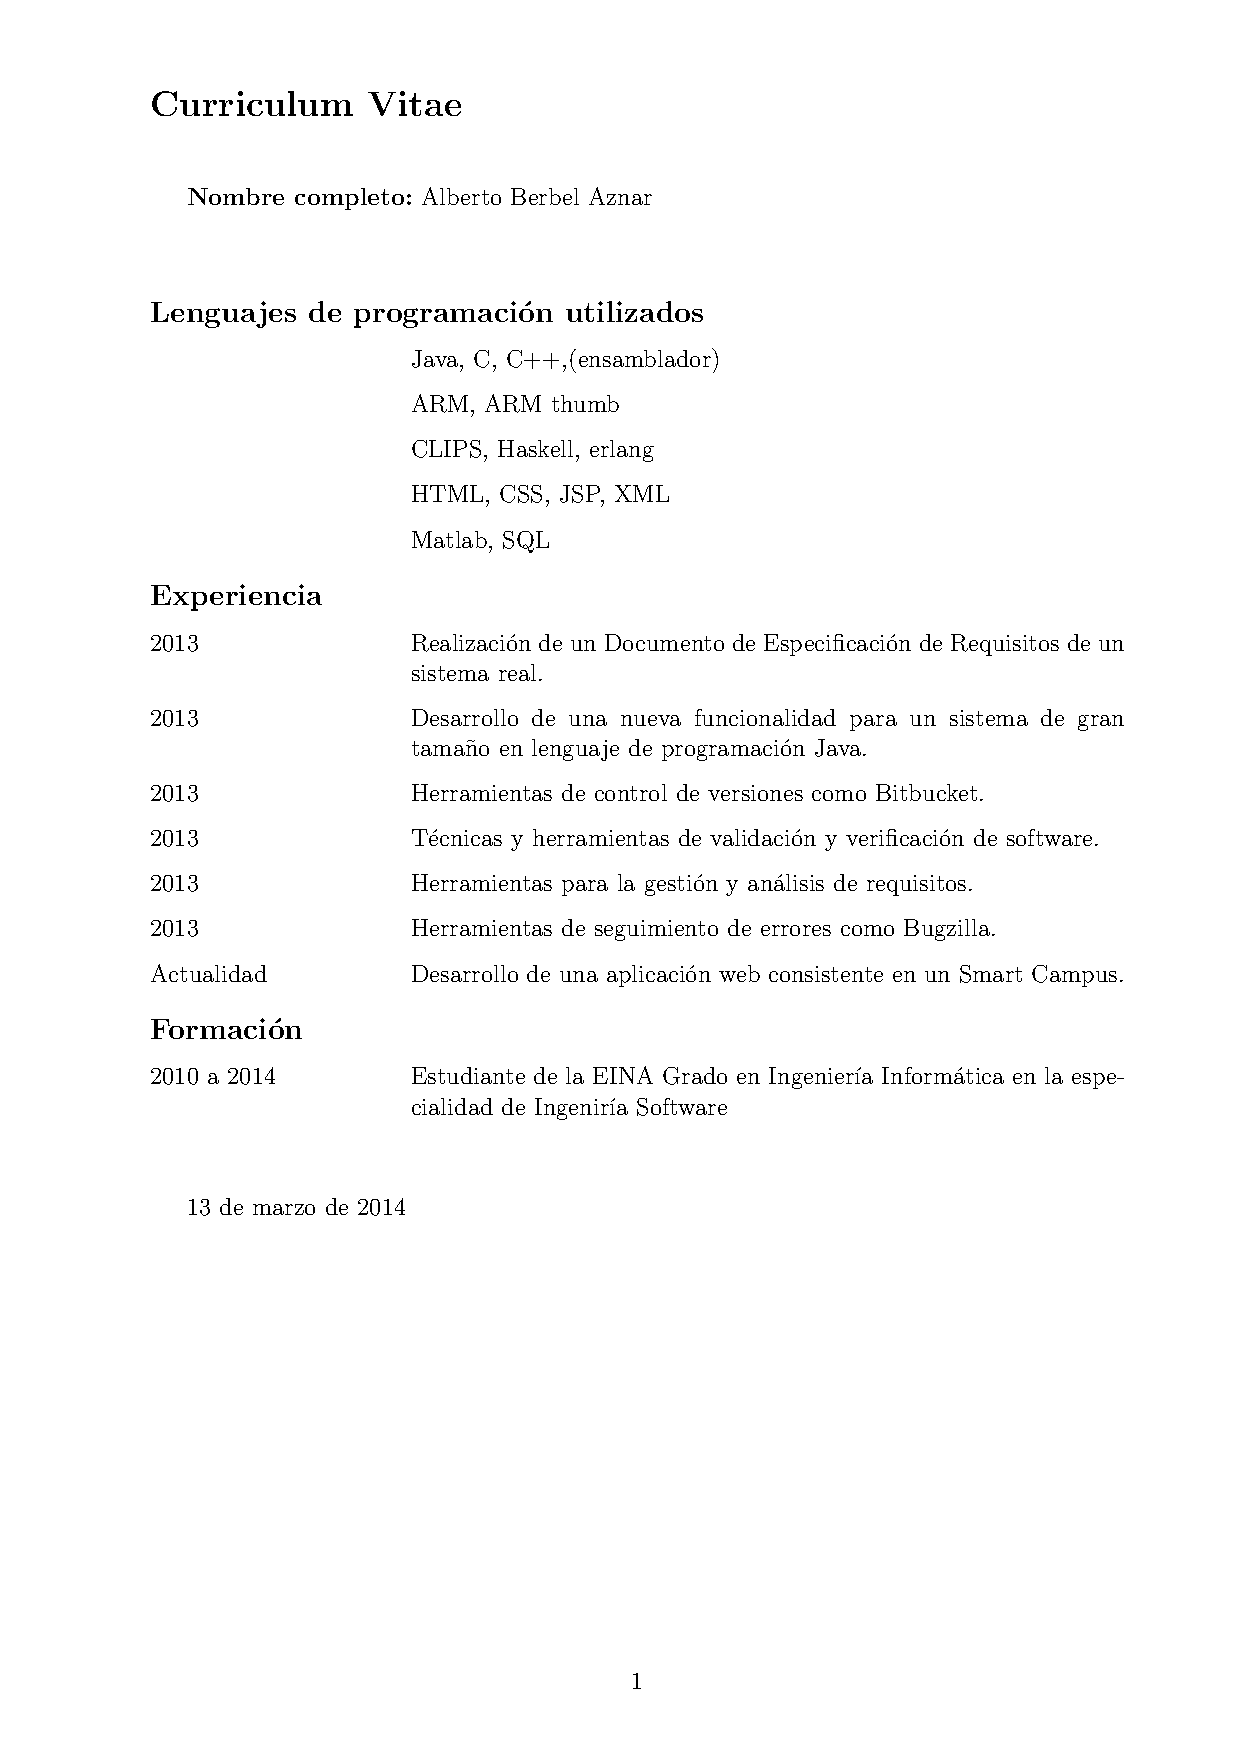
\includepdf[pages={1}]{cv_pdf/alberto_cv.pdf}
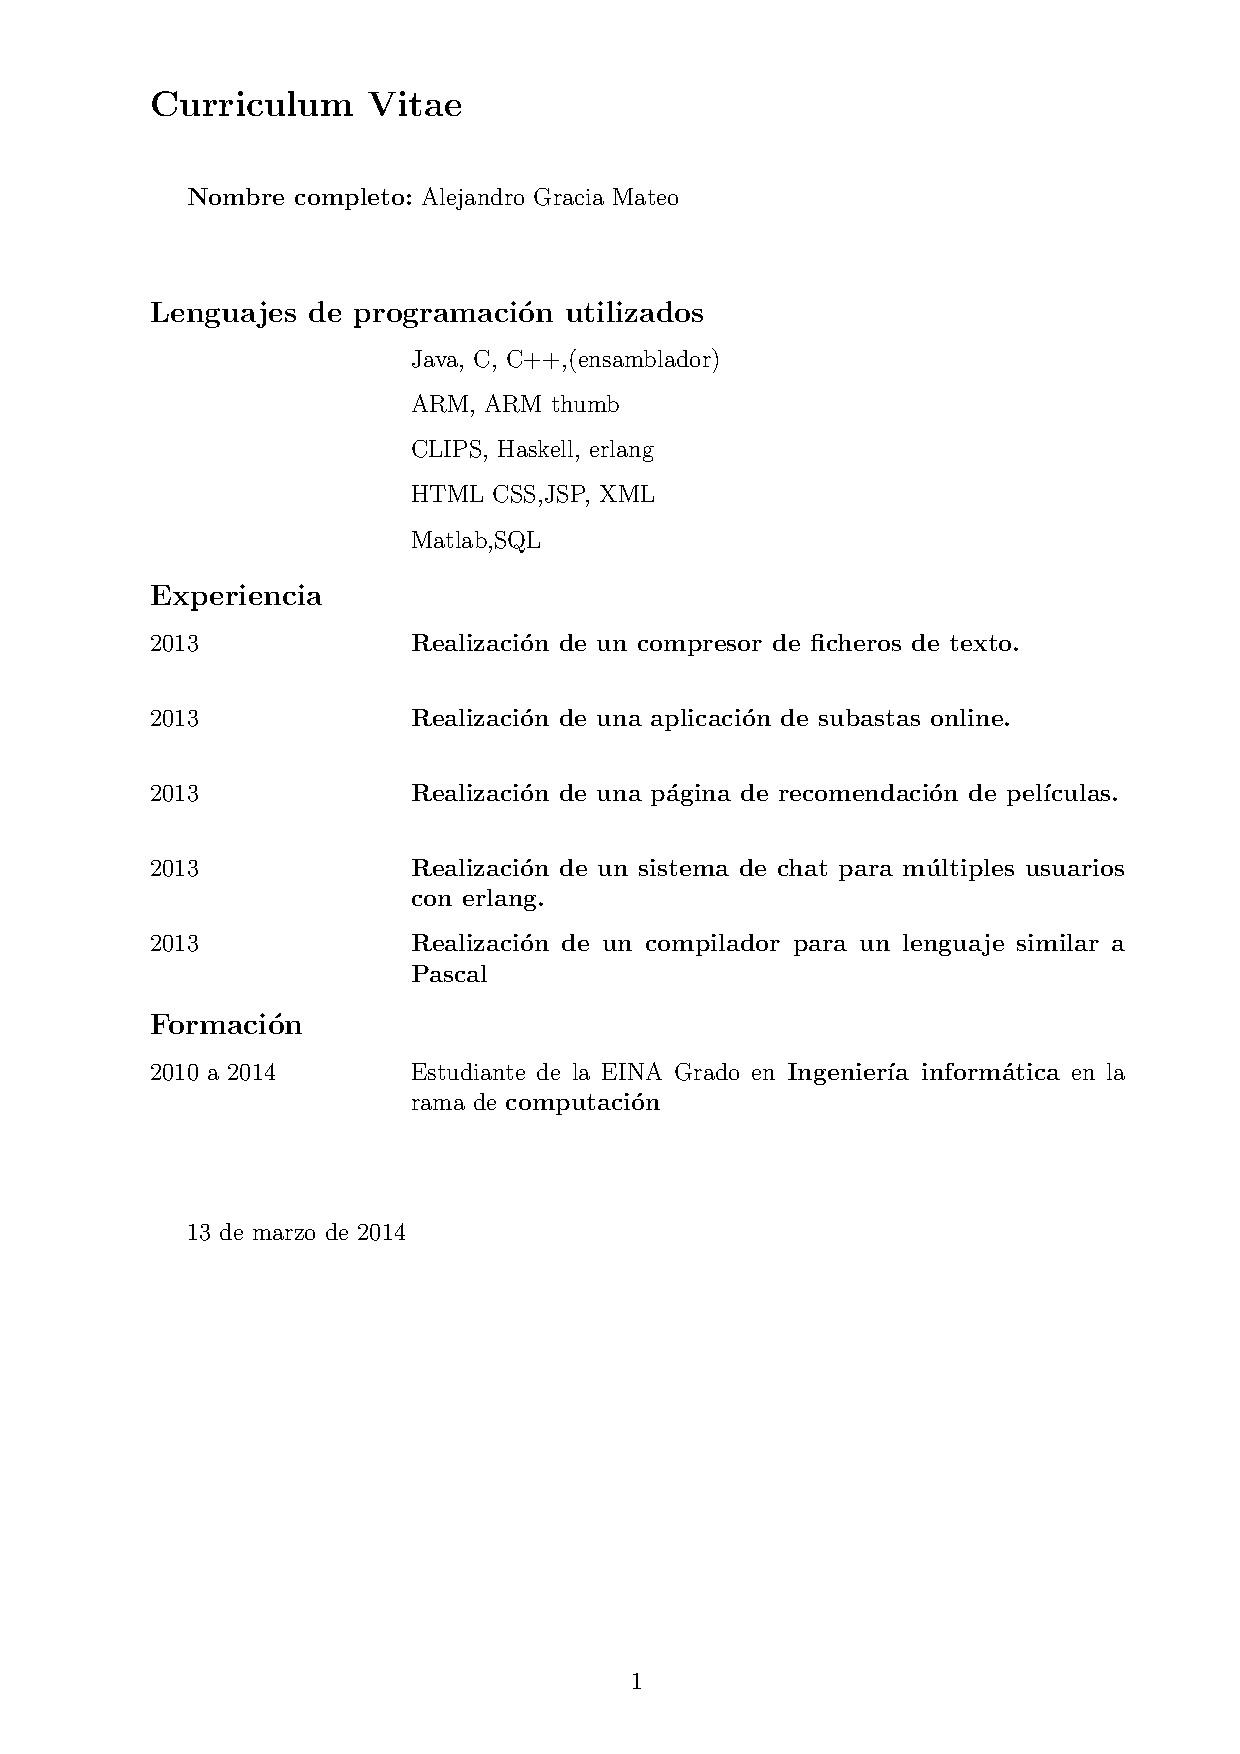
\includepdf[pages={1}]{cv_pdf/alejandro_cv.pdf}
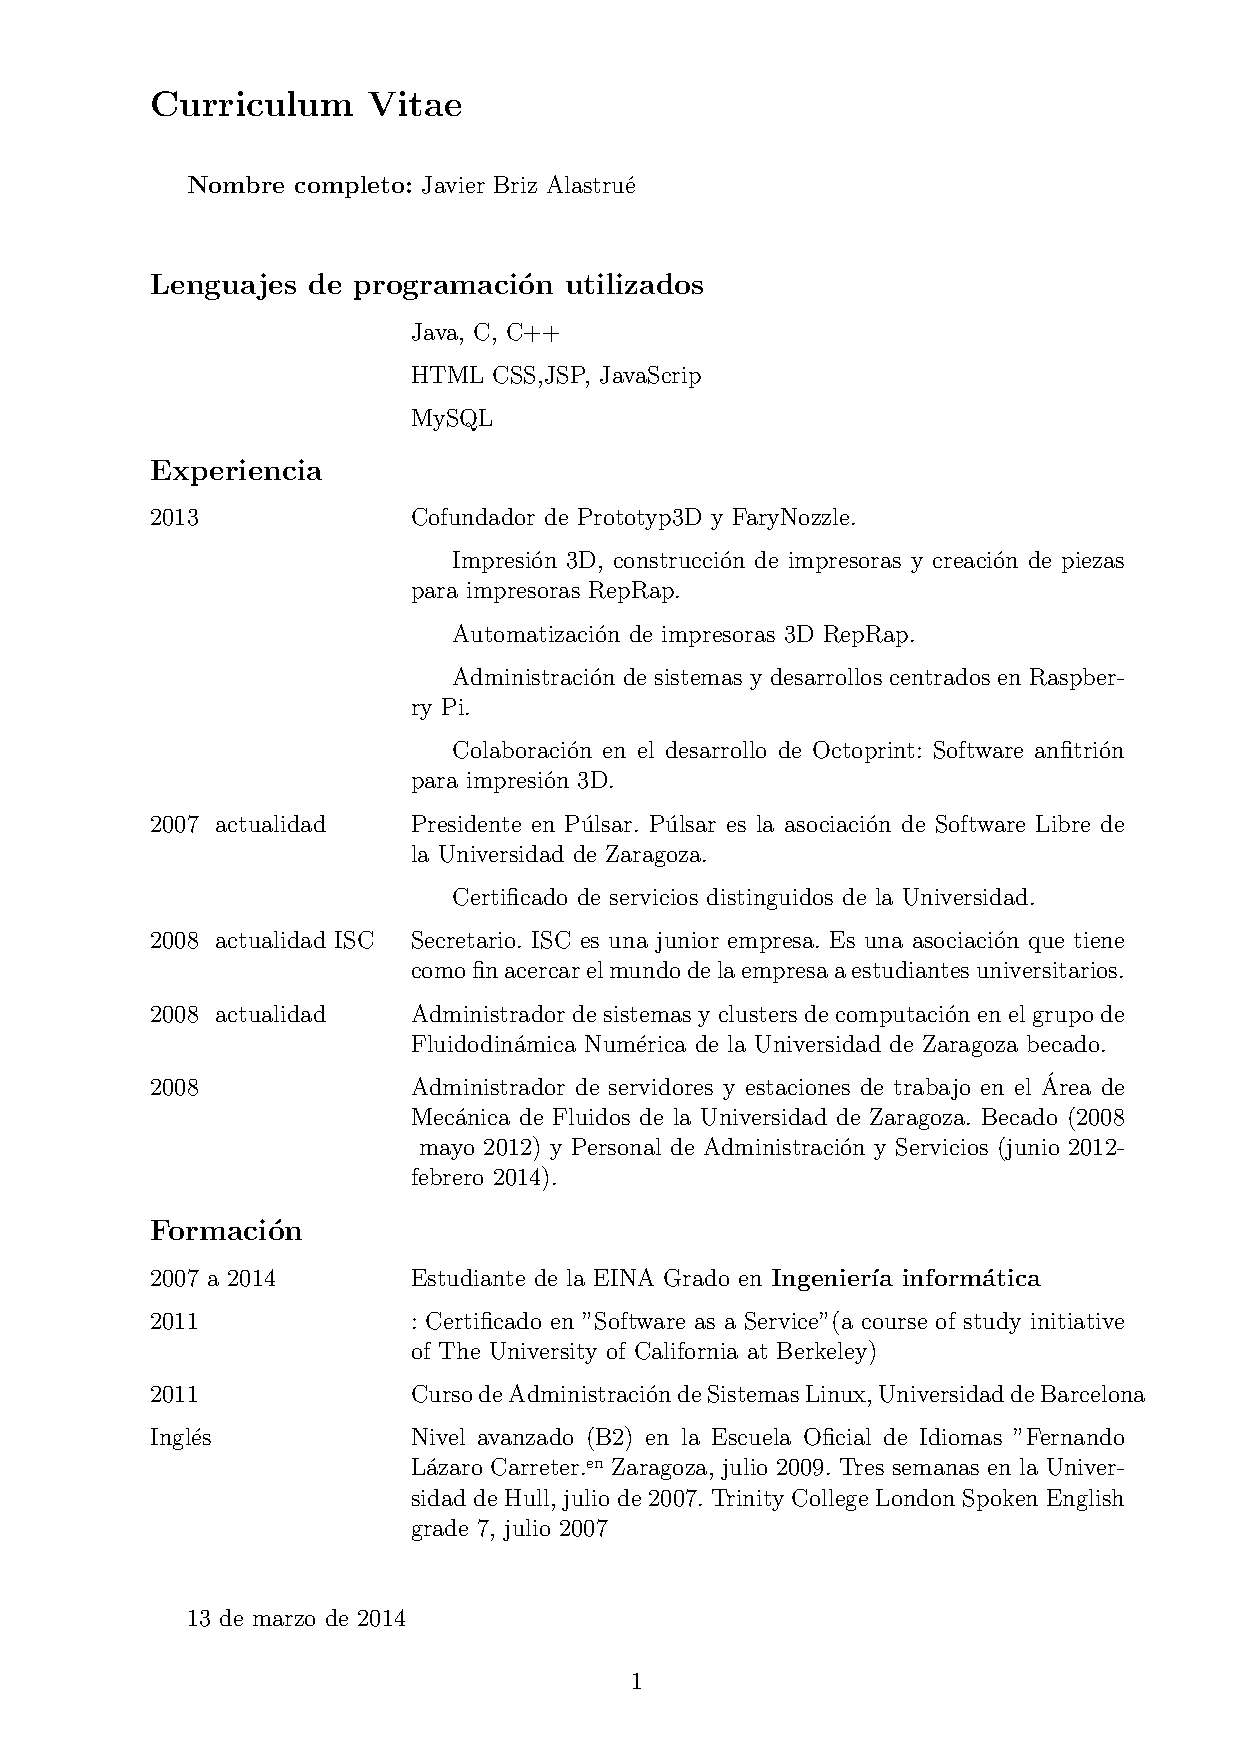
\includepdf[pages={1}]{cv_pdf/javier_cv.pdf}
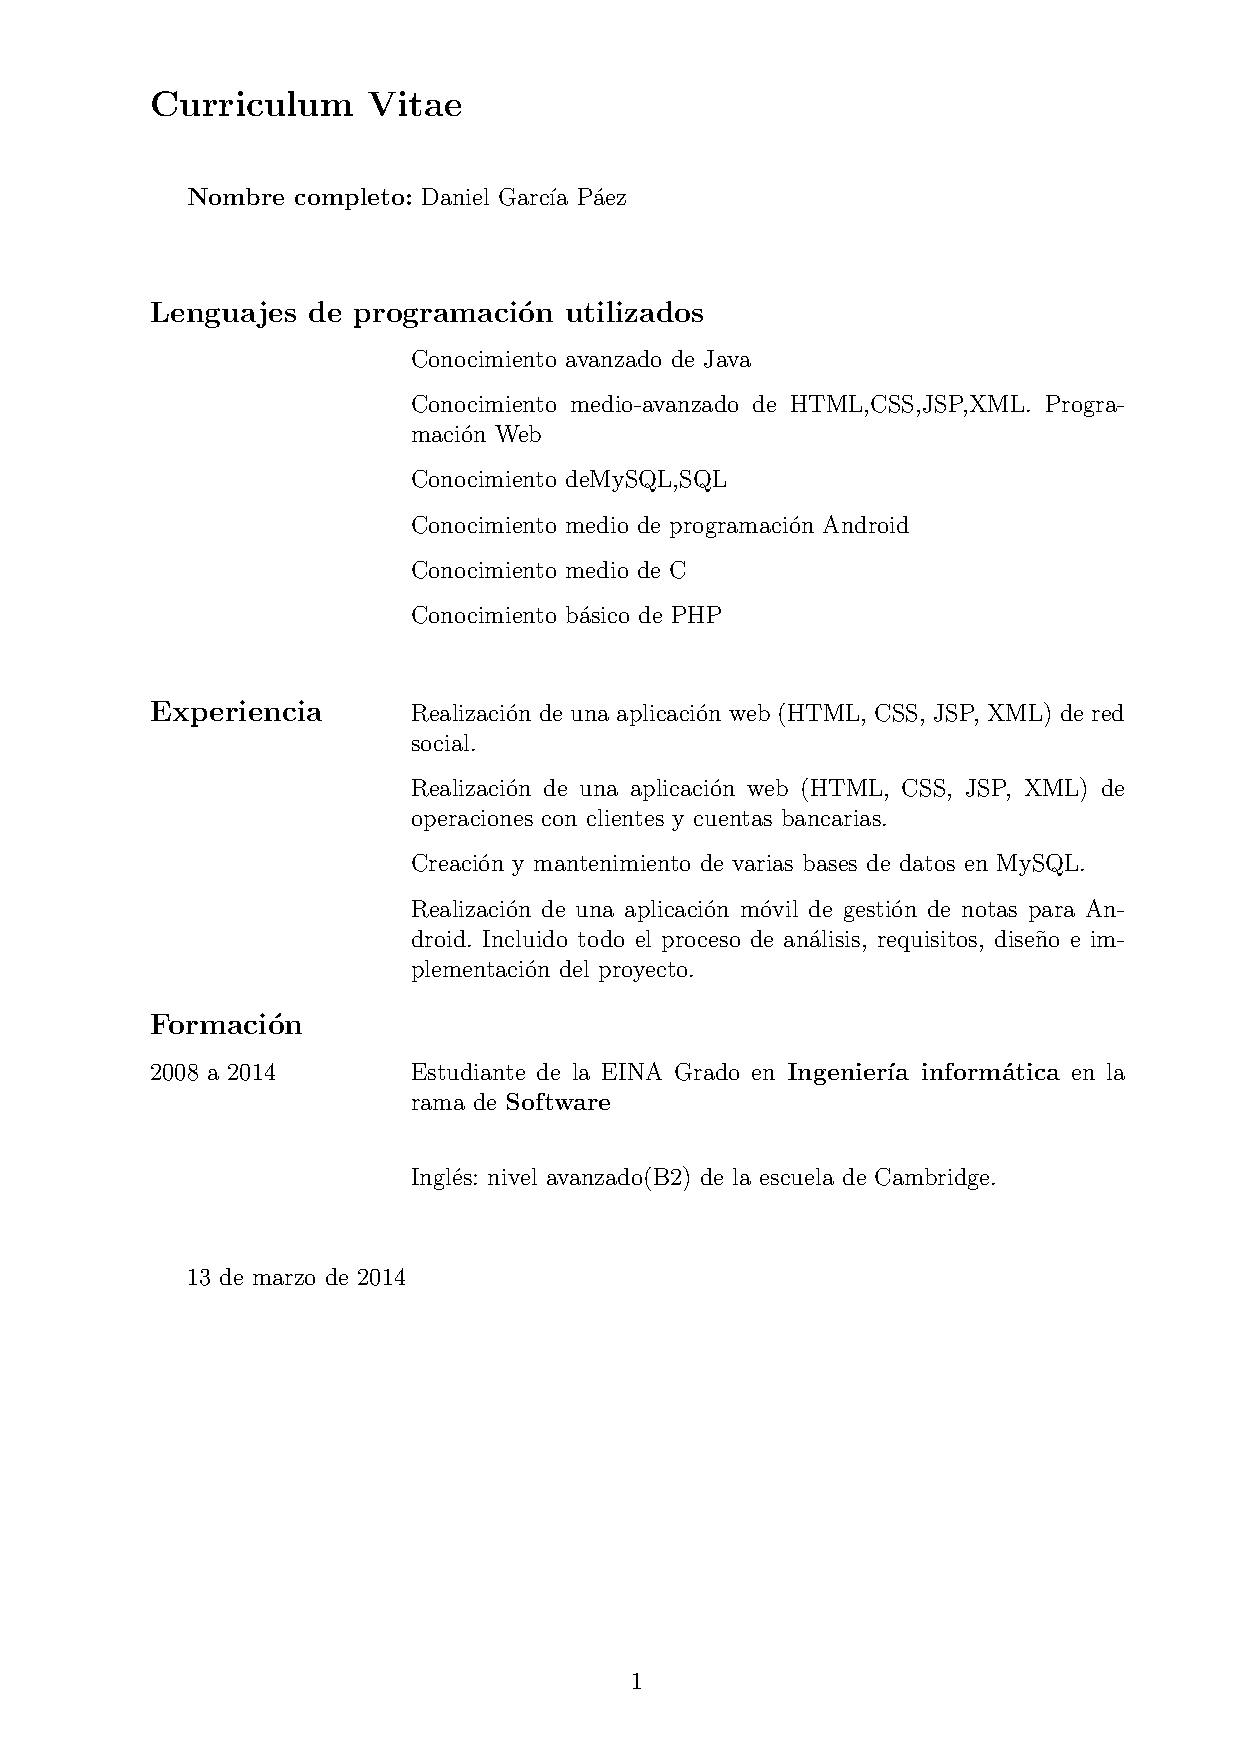
\includepdf[pages={1}]{cv_pdf/daniel_cv.pdf}
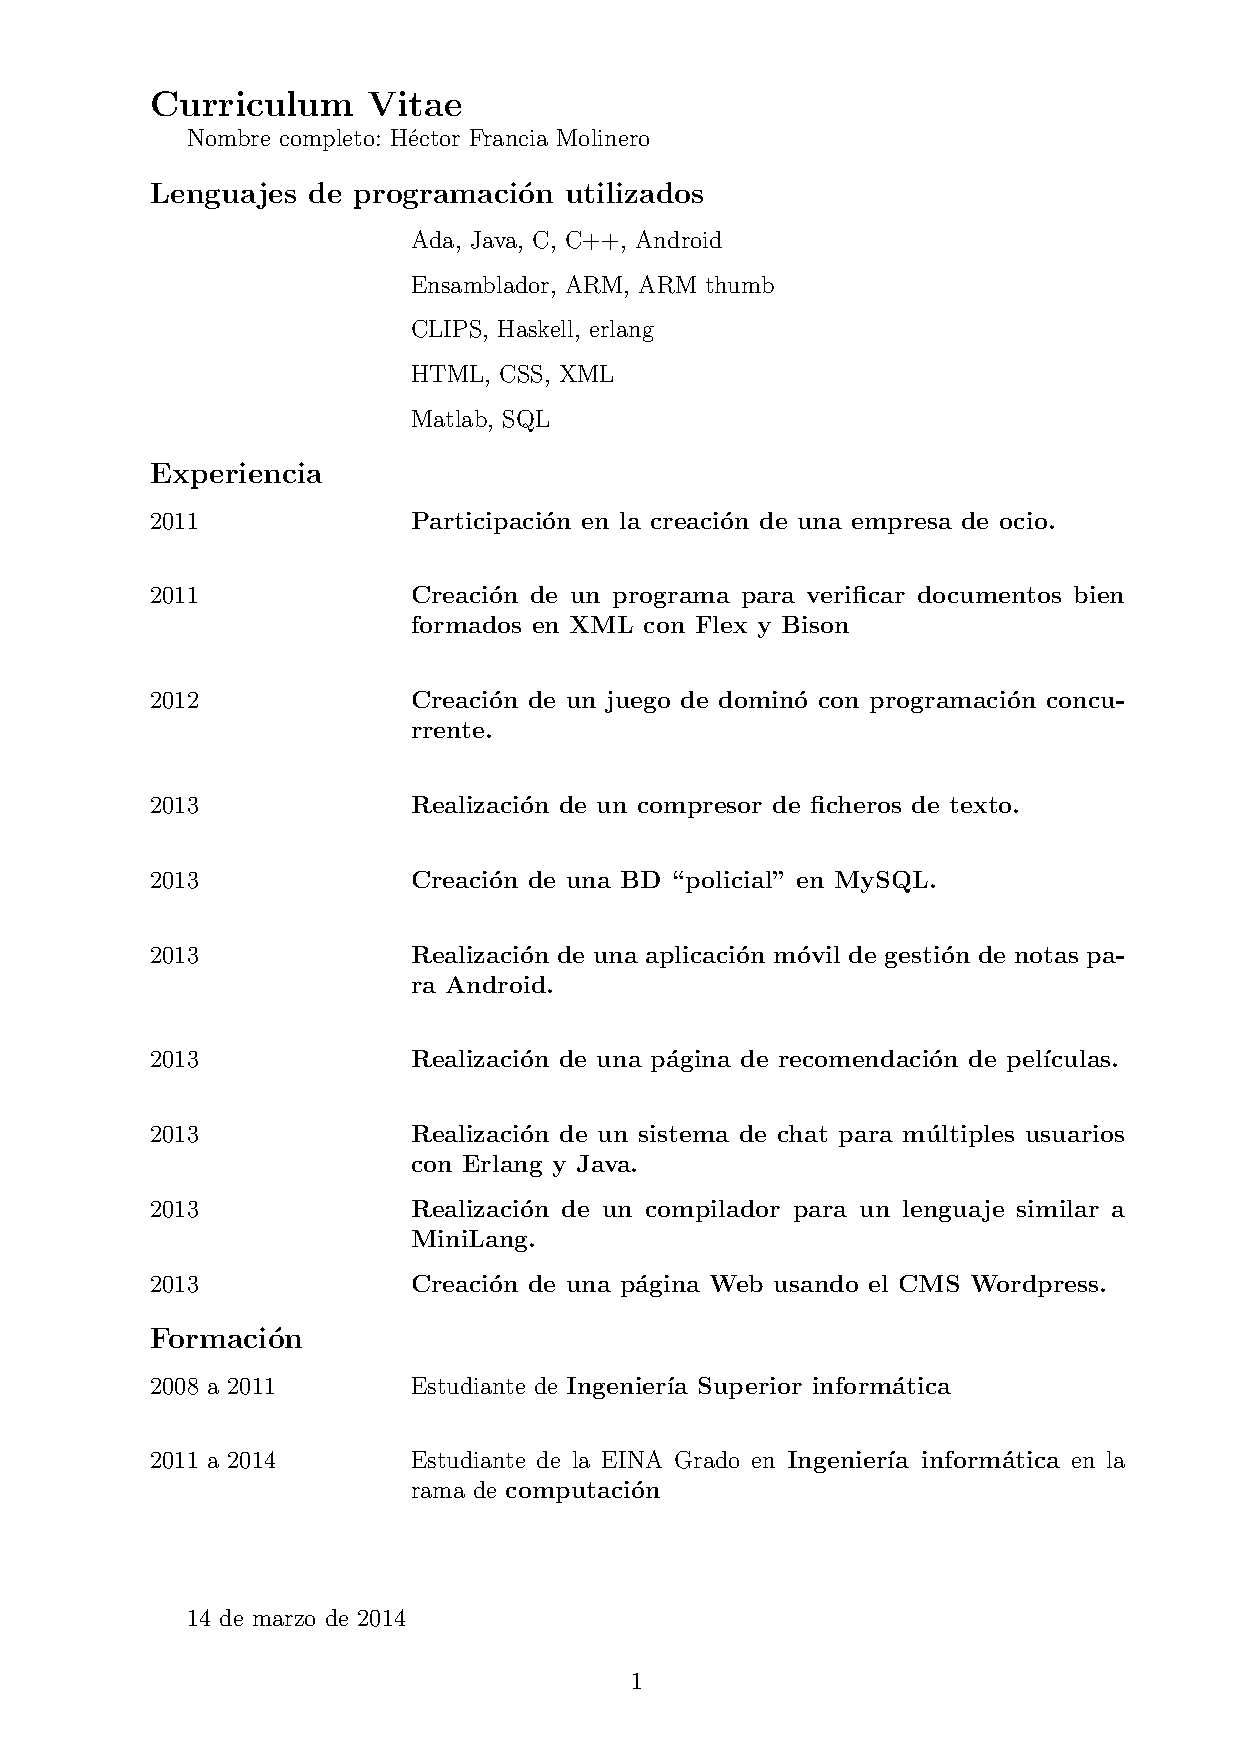
\includepdf[pages={1}]{cv_pdf/hector_cv.pdf}
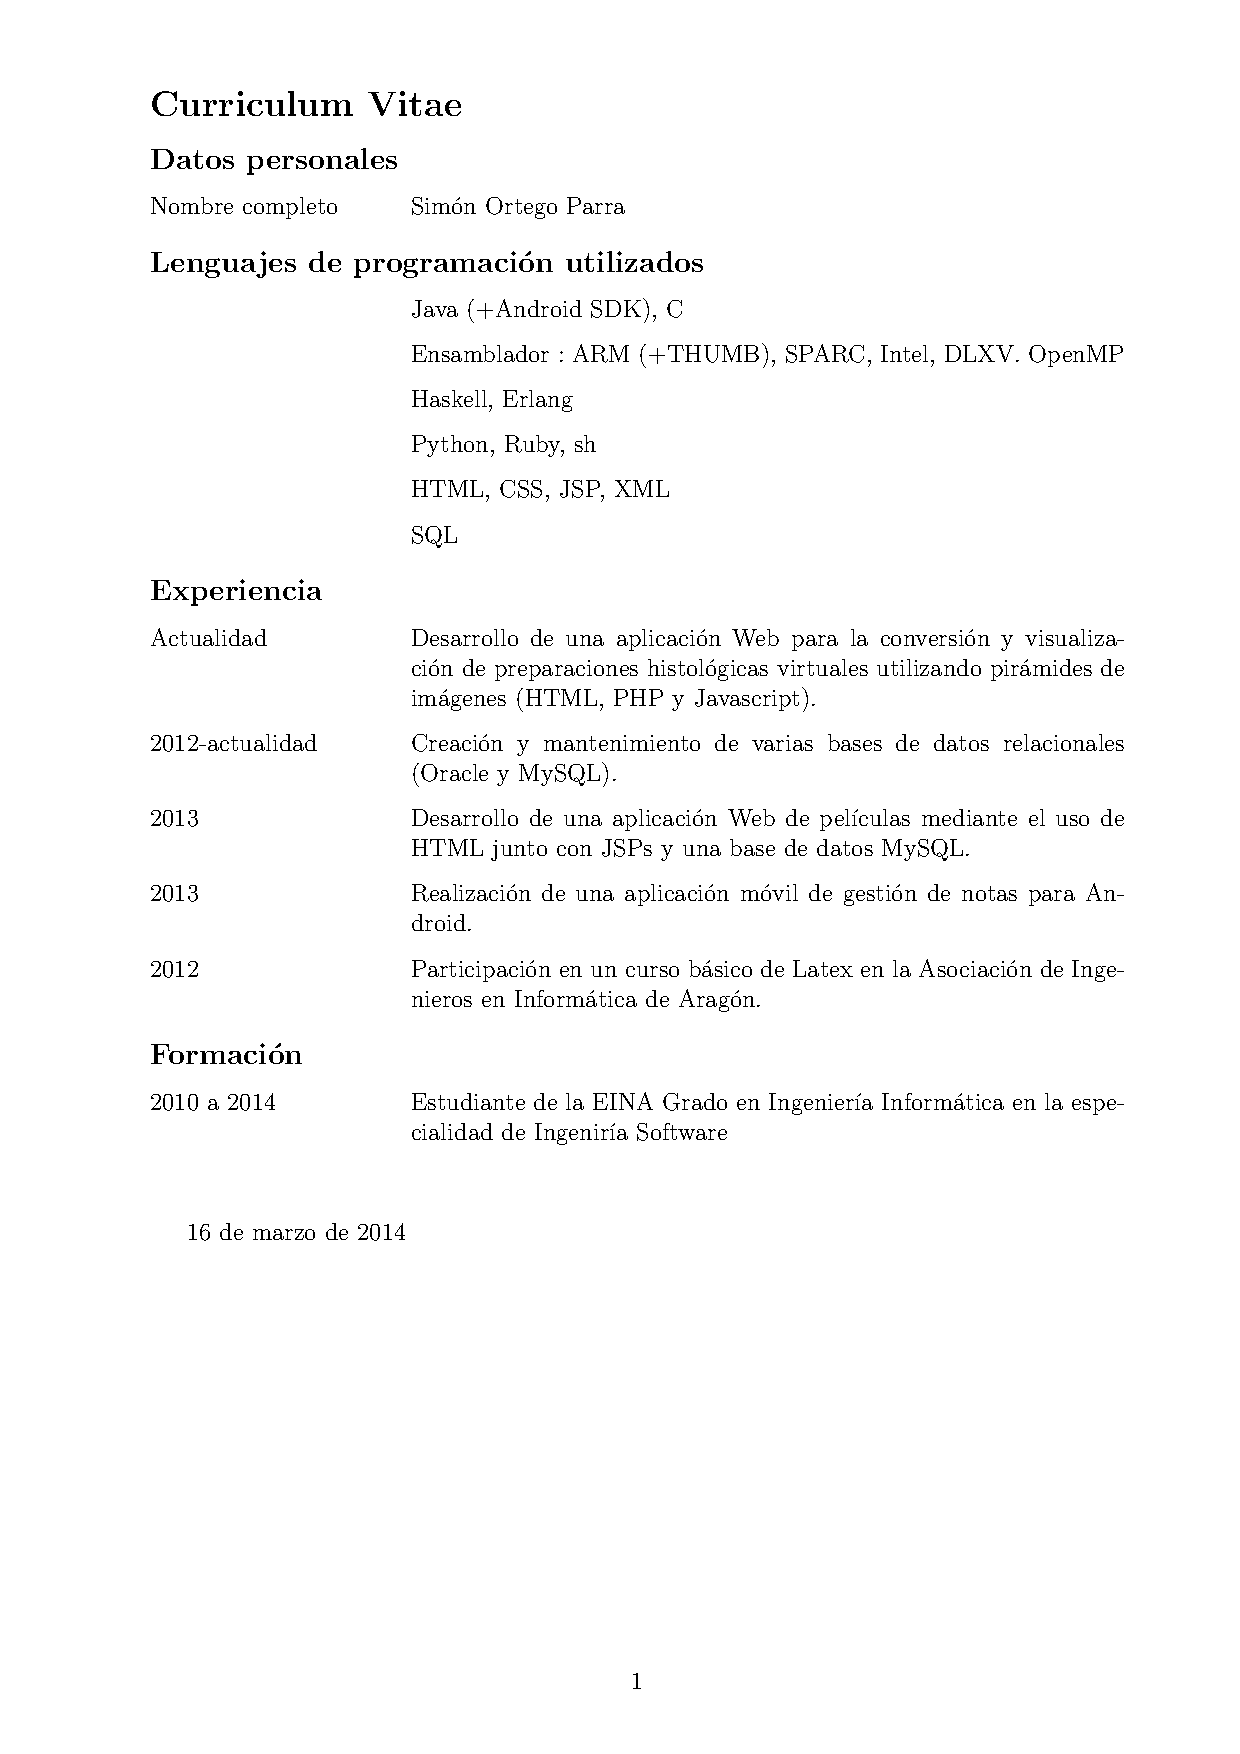
\includepdf[pages={1}]{cv_pdf/simon_cv.pdf}

\subsection{Cronograma}
En la~\cref{fig:diagGantt} se puede observar el calendario del proyecto con cada una de las
tareas repartidas en las dos iteraciones y con las fechas de entrega parciales correspondientes
a cada tarea.

\begin{sidewaysfigure}
\thisfloatpagestyle{empty} 
\centering
\scalebox{0.8}{
  \begin{gantt}[xunitlength=0.15cm,fontsize=\small,titlefontsize=\small,drawledgerline=true]{22}{150}
	  
    \begin{ganttitle} % Primer título año: 2014
      \titleelement{2014}{150}
    \end{ganttitle}
	
    \begin{ganttitle} % Segundo título meses: Ene-Junio
	  \titleelement{Febrero}{28}
	  \titleelement{Marzo}{31}
	  \titleelement{Abril}{30}
	  \titleelement{Mayo}{31}
	  \titleelement{Junio}{30}
    \end{ganttitle}
	
    \begin{ganttitle} % Tercer título fechas importantes
	  \titleelement{ }{25}
	  \titleelement{28}{3}
	  \titleelement{ }{7}
	  \titleelement{10}{3}
	  \titleelement{ }{7}
	  \titleelement{20}{3}
	  \titleelement{ }{4}
	  \titleelement{27}{3}
	  \titleelement{ }{13}
	  \titleelement{10}{3}
	  \titleelement{ }{11}
	  \titleelement{24}{3}
	  \titleelement{ }{13}
	  \titleelement{8}{2}
	  \titleelement{ }{5}
	  \titleelement{15}{3}
	  \titleelement{ }{9}
	  \titleelement{26}{3}
	  \titleelement{ }{3}
	  \titleelement{2}{3}
	  \titleelement{ }{24}
    \end{ganttitle}
	
	\ganttgroup{1\textsuperscript{a} iteración}{26}{58}
    \ganttbar[color=verde_cronograma]{Tarea 0}{25}{13}
	\ganttbar[color=rojo_cronograma]{Tarea 1}{38}{10}
	\ganttbar[color=rojo_cronograma]{Población BD}{38}{10}
    \ganttbar[color=azul_cronograma]{Tarea 2}{48}{7}
	\ganttbar[color=azul_cronograma]{Tarea 3}{48}{7}
    \ganttbar[color=azul_cronograma]{Tarea 4}{48}{7}
	\ganttbar[color=azul_cronograma]{Tarea 5}{48}{7}
	\ganttbar[color=naranja_cronograma]{Doc. técnica}{48}{23}
	\ganttbar[color=fucsia_cronograma]{Guía de Usuario}{71}{14}
	\ganttbar[color=gris_cronograma]{Pruebas}{55}{30}
	
	\ganttgroup{2\textsuperscript{a} iteración}{86}{40}
    \ganttbar[color=verde_cronograma]{Tarea 6}{85}{15}
	\ganttbar[color=verde_cronograma]{Tarea 7}{85}{15}
    \ganttbar[color=rojo_cronograma]{Tarea 8}{85}{23}
	\ganttbar[color=rojo_cronograma]{Doc. técnica}{85}{23}
	\ganttbar[color=azul_cronograma]{Guía de Usuario}{108}{13}
	\ganttbar[color=naranja_cronograma]{Pruebas}{100}{21}
	\ganttbar[color=fucsia_cronograma]{Cierre}{121}{6}
	
  \end{gantt}
}
\caption{Diagrama de Gantt que ilustra el calendario del proyecto}
\label{fig:diagGantt}
\end{sidewaysfigure}

\subsection{Presupuesto}
\paragraph{}Se presenta a continuación la propuesta de presupuesto u oferta económica:

D.DANIEL GARCÍA PÁEZ, D.JAVIER BRIZ ALASTRUE, D.SIMÓN ORTEGO PARRA, D.ALBERTO BERBEL AZNAR, D.HÉCTOR FRANCIA MOLINERO y D.ALEJANDRO GRACIA MATEO, domiciliados para estos efectos en Zaragoza, provincia de Zaragoza, calle Maria Luna número 3, en nombre y representación de la empresa BITPARTY S.L. con domicilio fiscal en Zaragoza, calle Maria Luna número 3, enterada del anuncio publicado en el “B.O.E.” del día 10 de FEBRERO de 2014 y de las condiciones y requisitos que se exigen para la adjudicación de los servicios de la creación de una aplicación web para la venta de microcontroladores a través de un catálogo electrónico, provincia de ZARAGOZA, se compromete a tomar a su cargo la ejecución de los mismos, con estricta sujeción a los requisitos y condiciones expresados, por las cantidades que se enumeran en concepto de precio, indicándose igualmente el IVA a soportar por la Administración, en cada caso, según las soluciones siguientes:

\begin{table}[h]
\begin{tabular}{|c|c|c|}
\hline
\multirow{3}{*}{SOLUCION}                              & \multicolumn{2}{|c|}{CANTIDAD}\\
\cline{2-3}
                                                       & \multicolumn{2}{|c|}{EUROS} \\
\cline{2-3}
                                                       & EN LETRA                                                                                                                    & EN NÚMERO   \\
\hline
\begin{tabular}[|c|]{@{}c@{}}BASE\\ Precio\end{tabular}  & \begin{tabular}[|c|]{@{}c@{}}Catorce mil novecientos cuarenta\\ y dos euros con ochenta\\ y dos céntimos de euro\end{tabular} & 14.942,82 \euro \\
\hline
IVA Admón.                                             & \begin{tabular}[|c|]{@{}c@{}}Tres mil ciento treinta\\ y ocho euros\end{tabular}                                              & 3.138,00 \euro  \\
\hline
\begin{tabular}[|c|]{@{}c@{}}TOTAL\\ Precio\end{tabular} & \begin{tabular}[|c|]{@{}c@{}}Dieciocho mil ochenta euros\\ con ochenta y dos\\ céntimos de euro\end{tabular}                  & 18.080,82 \euro \\
\hline
\end{tabular}
\end{table}

El licitador hace constar que el precio o precios del contrato ofertado incluyen el importe de las tasas
que sean de aplicación, con conformidad con lo señalado en el Pliego de Claúsulas Administrativas
Particulares que rige este contrato.
El licitador hace constar que el precio ofertado será pagado en dos plazos, correspondientes con las
dos iteraciones en las que el proyecto será realizado, de la siguiente manera:

\begin{table}[h]
\begin{tabular}{|c|c|c|}
\hline
\multirow{3}{*}{SOLUCION} & \multicolumn{2}{|c|}{CANTIDAD}                                                                                                             \\
\cline{2-3}
                          & \multicolumn{2}{|c|}{EUROS}                                                                                                                \\
\cline{2-3}
                          & EN LETRA                                                                                                                   & EN NÚMERO   \\
\hline
PAGO 1ª ITERACIÓN         & \begin{tabular}[c]{@{}c@{}}Once mil trescientos noventa\\ y cuatro euros con treinta\\ y dos céntimos de euro\end{tabular} & 11.394,32 € \\
\hline
PAGO 2ª ITERACIÓN         & \begin{tabular}[c]{@{}c@{}}Seis mil seiscientos ochenta\\ y seis euros con cincuenta\\ céntimos de euro\end{tabular}       & 6.686,50 € \\
\hline
\end{tabular}
\end{table}


\end{document}
